\section{不定积分}

本节给出不定积分这个概念,这个概念完全是为了求解定积分,将定积分的求解过程中的求原函数步骤独立出来研究,讨论各种方法(换元法、凑微法、部分积分法等)。

本节要点:
\begin{itemize}
    \item 掌握不定积分的计算方法。
\end{itemize}

%============================================================
\subsection{不定积分的概念}

\begin{definition}[不定积分]
若某区间上$F\left( x \right) $是$f\left( x \right) $的一个原函数,则$f\left( x \right) $所有原函数的一般表达式$F\left( x \right) +C$称为{\bf $f\left( x \right) $的不定积分(indefinite function)},记为$\int{f\left( x \right) dx}$,即:
\[
\int{f\left( x \right) dx}:=F\left( x \right) +C
\]
其中:
\begin{itemize}
    \item $x$:积分变量;
    \item $f\left( x \right) $:被积函数;
    \item $f\left( x \right) dx$:积分表达式。
\end{itemize}
\end{definition}

定积分可以理解为不定积分在一段区间内的变化量。

%============================================================
\subsection{不定积分的几何意义}

\begin{figure}[h]
\centering
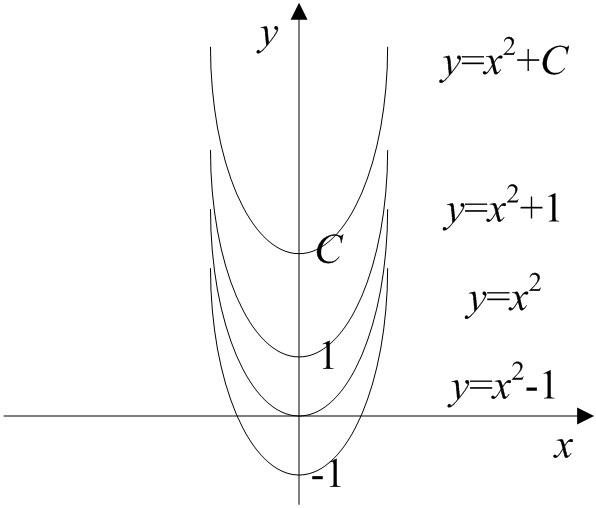
\includegraphics[height=4cm]{3.4.png}
\end{figure}

切线符合$y=x^2$的所有曲线的集合。

%============================================================
\subsection{不定积分的性质}

互逆运算:
\begin{align*}
&\left[ \int{f\left( x \right) dx} \right] '=f\left( x \right) \\
&\int{F'\left( x \right) dx}=F\left( x \right) +C
\end{align*}

线性性:
\[
\int{\left[ mf\left( x \right) +ng\left( x \right) \right] dx}=m\int{f\left( x \right) dx}+n\int{g\left( x \right) dx}
\]

\begin{tcolorbox}
线性性对应着导数运算中的$\left( f\pm g \right) '=f'\pm g'$。
\end{tcolorbox}

%============================================================
\subsection{不定积分计算方法}

{\bf 换元法(凑微分法)}:设$u=u\left( x \right) $具有连续导数,$F\left( u \right) $是$f\left( u \right) $的一个原函数,则:
\[
\int{f\left( u \right) u'\left( x \right) dx}=\int{f\left( u \right) du}=F\left( u \right) +C=F\left[ u\left( x \right) \right] +C
\]

\begin{tcolorbox}
线性性对应着导数运算中的$\frac{dy}{dx}=\frac{dy}{du}\cdot \frac{du}{dx}$。
\end{tcolorbox}

常用换元公式:
\begin{align*}
&\int{f\left( ax+b \right) dx}=\frac{1}{a}\int{f\left( ax+b \right) d\left( ax+b \right)} \quad a\ne 0 \\
&\int{f\left( x^a \right) x^{a-1}dx}=\frac{1}{a}\int{f\left( x^a \right) d\left( x^a \right)} \quad a\ne 0 \\
&\int{f\left( e^x \right) e^xdx}=\int{f\left( e^x \right) d\left( e^x \right)} \\
&\int{f\left( \ln x \right) \frac{1}{x}dx}=\int{f\left( \ln x \right) d\left( \ln x \right)} \\
&\int{\frac{\varphi '\left( x \right)}{\varphi \left( x \right)}dx}=\int{\frac{1}{\varphi \left( x \right)}d\varphi \left( x \right)}=\ln \left| \varphi \left( x \right) \right|+C
\end{align*}

~

{\bf 部分积分法}:设$u\left( x \right) ,v\left( x \right) $都具有连续导数,则:
\[
\int{uv'dx}=uv-\int{u'vdx} \quad \text{或写成} \quad \int{udv}=uv-\int{vdu}
\]

\begin{tcolorbox}
部分积分法和微分中的导数运算法则对应,$\left( fg \right) '=f'g+fg'$。
\end{tcolorbox}

%============================================================
\subsection{基本积分公式}

\begin{align*}
&\int{0dx}=C \\
&\int{x^adx}=\frac{1}{a+1}x^{a+1}+C \quad a\ne -1 \\
&\int{\frac{1}{x}dx}=\ln \left| x \right|+C \\
&\int{a^xdx}=\frac{a^x}{\ln a}+C \quad a>0,a\ne -1 \\
&\int{e^xdx}=e^x+C \\
&\int{\cos xdx}=\sin x+C \\
&\int{\sin xdx}=-\cos x+C \\
&\int{\sec ^2xdx}=\tan x+C \\
&\int{\csc ^2xdx}=-\cot x+C \\
&\int{\sec x\tan xdx}=\sec x+C \\
&\int{\csc x\cot xdx}=-\csc x+C \\
&\int{\frac{1}{\sqrt{1-x^2}}dx}=\mathrm{arc}\sin x+C \\
&\int{\frac{1}{1+x^2}dx}=\mathrm{arc}\tan x+C
\end{align*}




